\chapter{Signal Analysis}
\paragraph{}  The large number of sensors and the rapid sampling of each sensor provides an enormous number of individual measurements of magnetic fields during the plasma's lifetime. The method of Biorthogonal Decomposition is used to isolate coherent fluctuations from this large dataset and provides an orthogonal basis set of modes, that are described in terms of their spatial shape and temporal evolution.  This chapter will describe the method of Biorthogonal Decomposition, how it is applied in this research, its strengths and limitations.

\section{The Biorthogonal Decomposition Algorithm}
\paragraph{}
The biorthogonal decomposition is used on non-square matrices, to produce a basis set of pseudo-eigenvalues and pseudo-eigenvectors.  A given matrix S is decomposed into 
\begin{equation}
A^{\intercal} A = U \Sigma V^{\intercal}
\end{equation}
Where the columns of U and the rows of V are orthogonal bases of the structures, however defined, that make up the rows and columns of the data. In this research, the rows are time series of individual sensor signals, with the signal across all sensors at any instant constituting the columns.  
$$
\begin{pmatrix}
\uparrow& &\uparrow\\
s_1&\cdots&s_N\\
\downarrow & &\downarrow
\end{pmatrix}
 =
\begin{pmatrix}
\uparrow& &\uparrow\\
u_1&\cdots&u_N\\
\downarrow & &\downarrow
\end{pmatrix}
\begin{pmatrix}
\sigma_1& &\\
&\ddots&\\
& &\sigma_N
\end{pmatrix}
\begin{pmatrix}
\leftarrow& v_1&\rightarrow\\
&\vdots&\\
\leftarrow& v_M &\rightarrow
\end{pmatrix}
$$



  can be derived by first multiplying the vector by its transpose.  The resulting matrix is square and is factorable into two independent sets of eigenvectors, which are related to the arrangement of column and row vectors.  
In the case of HBT-EP, the time-domain signal for each sensor is stitched together to give a matrix that has dimensions up to 216 X 5000.  There will be a set of eigenvalues equal in size to the smaller dimension.  The set of eigenvectors will be determined arbitrarily, with no a priori assumptions as to the form of the basis functions.  The only constraint is that they must all be orthogonal in both space and time.  That the poloidal modes do not form a clean Fourier basis set is therefore of no concern.  The toroidal and temporal structure, for which sinusoids are a good description, will allow for orthogonal bases which map well onto individual modes regardless of poloidal structure.  Thus modes with non-singular poloidal spectra can be adequately modeled, which would not be the case if a Fourier basis was used.
As seen in figure \ref{PA_sensors_top_3_modes} The signal of all sensors in a poloidal array is put through the BD, with the top three modes isolated.  The (exxagerated) amplitude is plotted on a poloidal cross section.  The development of each mode is clear, with some modes growing as time goes on, and others declining in amplitude.  The remaining signal shows some high wavenumber, low amplitude structure, but analysis of such low level signal can be difficult.


\begin{figure}
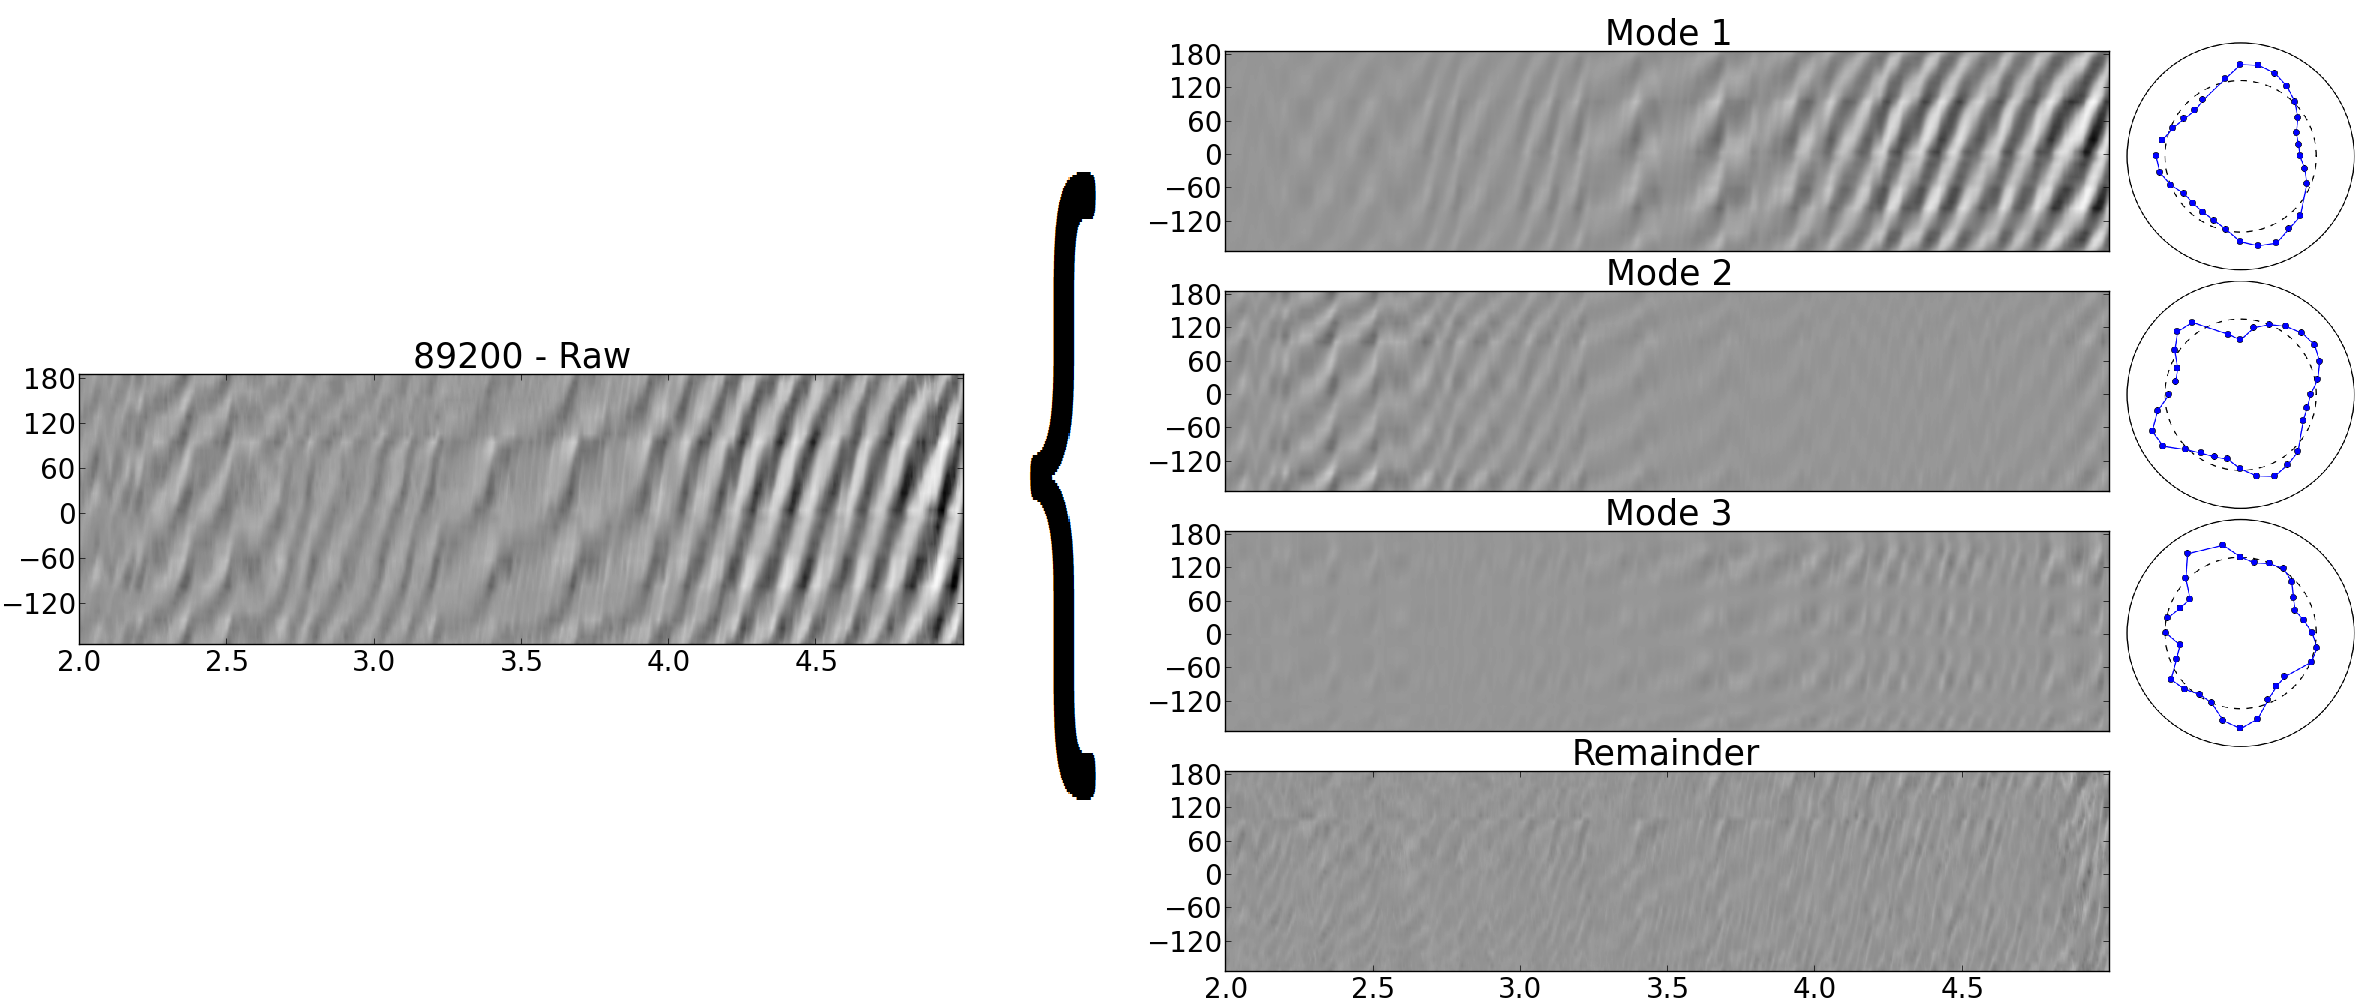
\includegraphics[width = \textwidth]{./figures/stripey_flucts_joined_grey_89200_mod.png}\begin{flushleft}
\caption{Greyscale contour plot of poloidal array raw signal, 3 dominant modes, and remainder of the full signal.  Mode structure is clearly visible, as is temporal evolution of mode amplitude.  Remainder shows structure - determining significance of low-order modes requires close analysis on a shot-by-shot basis}
\end{flushleft}
\label{PA_sensors_top_3_modes}
\end{figure}

